%%%%%%%%%%%%%%%%%%%%%%%%%%%%%%%%%%%%%%%%%
% Beamer Presentation
% LaTeX Template
% Version 1.0 (10/11/12)
%
% This template has been downloaded from:
% http://www.LaTeXTemplates.com
%
% License:
% CC BY-NC-SA 3.0 (http://creativecommons.org/licenses/by-nc-sa/3.0/)
%
%%%%%%%%%%%%%%%%%%%%%%%%%%%%%%%%%%%%%%%%%

%----------------------------------------------------------------------------------------
%	PACKAGES AND THEMES
%----------------------------------------------------------------------------------------



\documentclass[english]{beamer}

\mode<presentation> {

\usetheme{Madrid}

\usecolortheme[RGB={198, 0, 126}]{structure}


\setbeamertemplate{navigation symbols}{}
}
\usepackage[english, activeacute]{babel}
\usepackage[utf8]{inputenc} %Codificacion utf-8
\usepackage[official]{eurosym}
\usepackage{verbatim}

\usepackage{graphicx} % Allows including images
\usepackage{booktabs} % Allows the use of \toprule, \midrule and \bottomrule in tables


\useinnertheme{circles}
\newenvironment{proenv}{\only{\setbeamercolor{local structure}{fg=green}}}{}
\newenvironment{conenv}{\only{\setbeamercolor{local structure}{fg=red}}}{}



%----------------------------------------------------------------------------------------
%	TITLE PAGE
%----------------------------------------------------------------------------------------



\title[haspie]{Tool for musical harmonization\\through Answer Set Programming} 

\author[Rodrigo Martín Prieto]{Student:\\Rodrigo Martín Prieto}
\newcommand{\director}{Director:\\José Pedro Cabalar Fernández}
\institute[UDC] {
Universidade da Coruña \\ % Your institution for the title page
\medskip
\textit{r.martin@udc.es} % Your email address
}
\date{\today} % Date, can be changed to a custom date


\setbeamertemplate{title page}{
\centering
\vfill
\includegraphics[width=0.6\linewidth]{imagenes/anagramaUDC.png}
\vfill
\begin{beamercolorbox}[rounded=true,shadow=true,sep=8pt,center]{title}
\inserttitle \par
\end{beamercolorbox}
\vfill
\begin{beamercolorbox}[leftskip=8cm,center,wd=0.7\textwidth]{author}
\begin{columns}[T]
\begin{column}{.49\textwidth}%
\centering
\insertauthor
\end{column}
\begin{column}{.49\textwidth}%
\centering
\director
\end{column}
\end{columns}
\end{beamercolorbox}
\centering
\vfill
\insertdate\par
\vfill
}



\begin{document}

\begin{frame}
\titlepage % Print the title page as the first slide
\end{frame}

%----------------------------------------------------------------------------------------
%	PRESENTATION SLIDES
%----------------------------------------------------------------------------------------

\section{Motivation}
\begin{frame}
	\frametitle{Motivation}
			\begin{beamercolorbox}[leftskip=8cm,center,wd=0.7\textwidth]{author}
			\begin{columns}[T]
			\begin{column}{.60\textwidth}%
				\begin{itemize}
						\item Musical teaching is still very traditional nowadays.
						\item Self-teaching of music theory is hard.
						\item There aren't many tools to aid and guide students and self-taught students.
						\item Composition tools seek results assuming that the user knows musical theory.
				\end{itemize}
			\end{column}
			\begin{column}{.39\textwidth}%
			\includegraphics[width=\linewidth]{imagenes/music_theory.jpg}
			\end{column}
			\end{columns}
			\end{beamercolorbox}

\end{frame}

\subsection{Background}
\begin{frame}
	\frametitle{ANTON}
	\begin{itemize}
		\item ANTON [Bra10] is a full-fledged composition tool written in ASP
		\item Limited to choral pieces for two voices
		\item Only Giovanni Perluigi da Palestrina's style
	\end{itemize}
\end{frame}

\subsection{Goals}
	\begin{frame}
		\frametitle{Goals}
			\begin{beamercolorbox}[leftskip=8cm,center,wd=0.7\textwidth]{author}
			\begin{columns}[T]
			\begin{column}{.60\textwidth}%
				\begin{enumerate}
							\item Harmonize and annotate chords over any musical score
							\item Given a certain harmonization, be able to complete any incomplete voice of the score
							\item Complete on purpose blank sections of incomplete voices of the score
							\item Add new voices that complement the voices already in the score
						\end{enumerate}
			\end{column}
			\begin{column}{.39\textwidth}%
			\includegraphics[width=\linewidth]{imagenes/Beethoven.jpg}
			\end{column}
			\end{columns}
			\end{beamercolorbox}
	\end{frame}

\section{Musical Introduction}
\begin{frame}
	\frametitle{Overview}
	\tableofcontents[currentsection,subsections,hideothersubsections]
\end{frame}
\subsection{Figures and Rhythm}
	\begin{frame}
		\frametitle{Figures and Rhythm}
		\begin{beamercolorbox}[leftskip=8cm,center,wd=0.7\textwidth]{author}
		\begin{columns}[T]
		\begin{column}{.60\textwidth}%
		\begin{itemize}
			\item Every note is represented by a figure that determines it's length
			\item Each figure can be subdivided in two
			\item Rhythm is created by combining figures of different lengths with special symbols called silences
		\end{itemize}
		\end{column}
		\begin{column}{.39\textwidth}%
		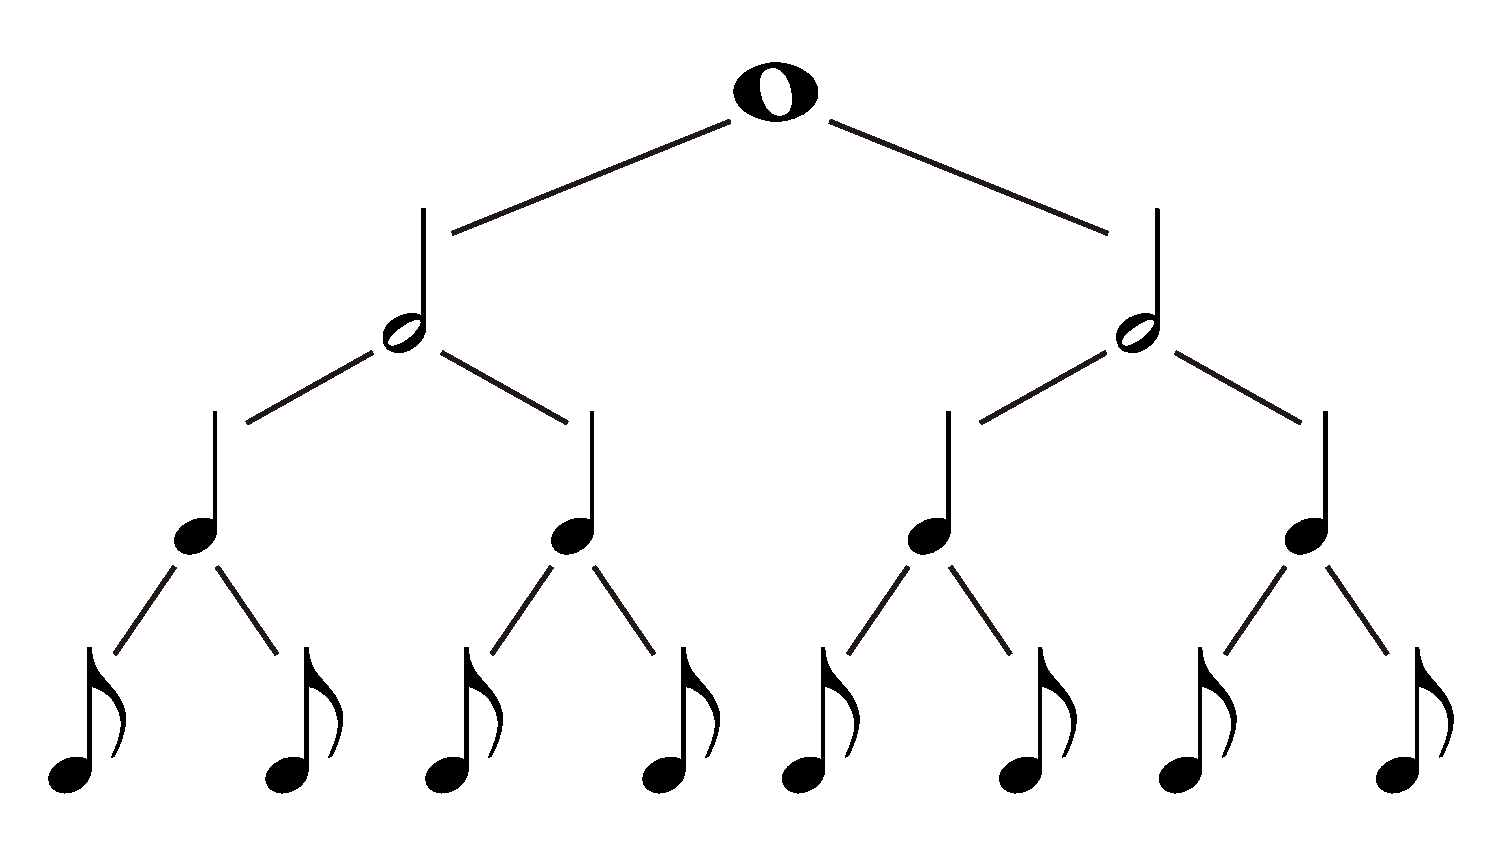
\includegraphics[width=\linewidth]{imagenes/music_tree.pdf}
		\end{column}
		\end{columns}
		\end{beamercolorbox}
		
	\end{frame}
\subsection{Melody}
	\begin{frame}
		\frametitle{Melody}
		\begin{itemize}
			\item Horizontal dimension of music
			\item Pitch is represented by the height at which the note is written, higher position means higher pitch
			\item The pitch of a note matters in relation to the adjacent notes
		\end{itemize}
		\begin{center}
			\includegraphics[width=0.6\linewidth]{imagenes/C_scale.png}
		\end{center}
	\end{frame}
\subsection{Harmony}
	\begin{frame}
		\frametitle{Harmony}
		\begin{itemize}
			\item Vertical dimension of music
			\item Only present in polyphonic pieces or pieces with polyphonic instruments
			\item The pitch of a note matters in relation to the notes above and below in the other voices
			\item Two notes of different voices that play at the same time form a chord
		\end{itemize}
		\begin{center}
			\includegraphics[width=0.6\linewidth]{imagenes/C_chords.png}
		\end{center}
		
	\end{frame}

\section{Demo}
\begin{frame}
	\frametitle{Overview}
	\tableofcontents[currentsection,subsections,hideothersubsections]
\end{frame}
	\begin{frame}
		\frametitle{Demonstration}
		The piece selected for the Demo will be Greensleeves by Henry VIII of England. We will see and hear the results of three diffrent processes performed by the tool.
		\begin{itemize}
			\item Harmonization and chord annotation of the score
			\item Given the previous harmonization, the tool will complete a section of the Cello part
			\item Given the previous harmonization, the tool will complete a section of the Violin part
		\end{itemize}
	\end{frame}

\section{The Project}
\begin{frame}
	\frametitle{Overview}
	\tableofcontents[currentsection,subsections,hideothersubsections]
\end{frame}
\subsection{Architecture}
	\begin{frame}
		\frametitle{haspie's Architecture}
		\begin{figure}
		\centering
		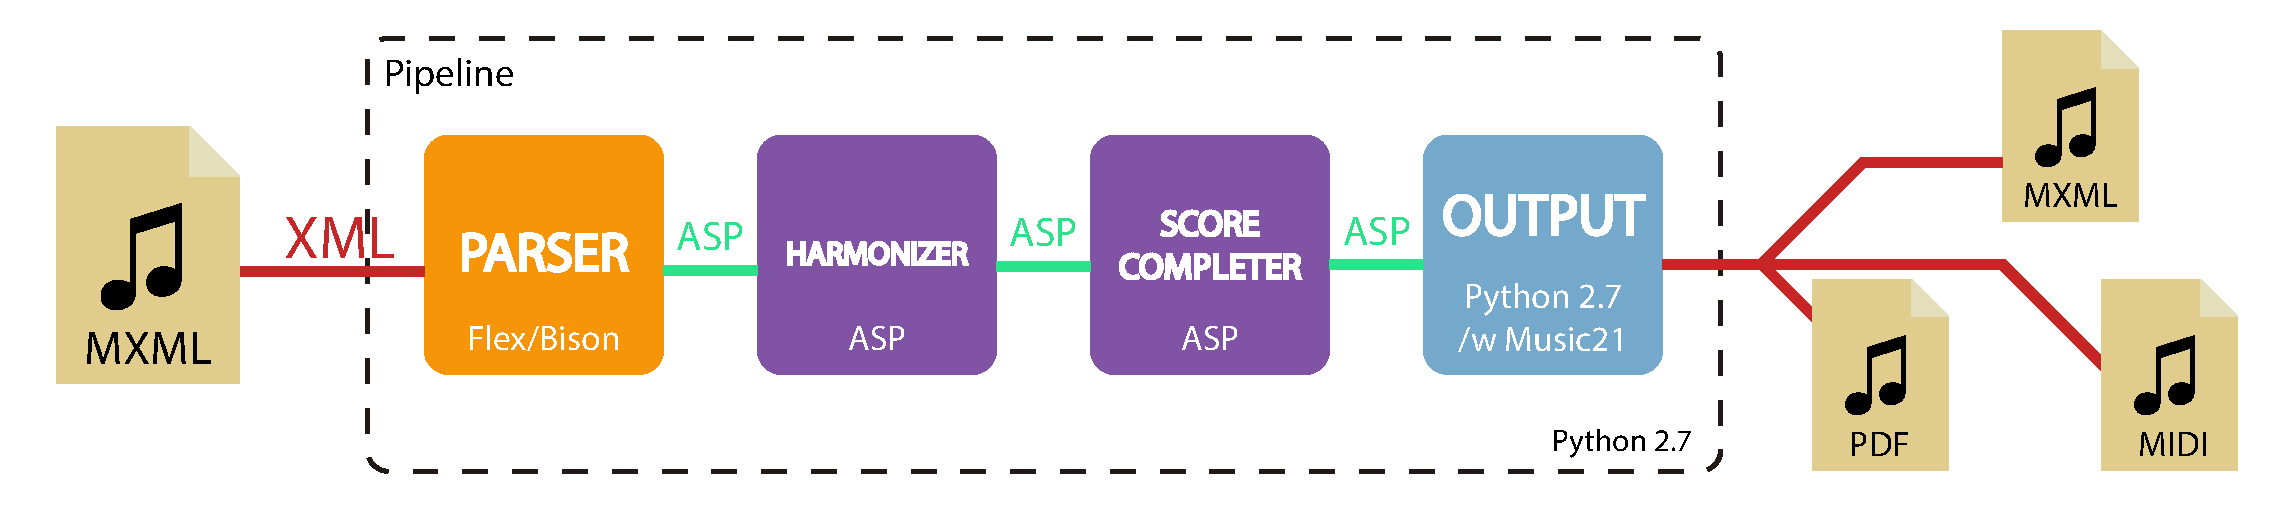
\includegraphics[width=\linewidth]{imagenes/arquitectura_final.pdf}
		\end{figure}
	\end{frame}
\subsection{ASP Core}
	\begin{frame}[t]
		\frametitle{The ASP Core}
		\begin{center}
		\includegraphics[width=0.6\linewidth]{imagenes/arch_trans/arquitectura_final_asp_core-01.png}
		\end{center}
		\begin{itemize}
			\item Independent of the solving process and its heuristics
			\item The power of ASP resides in this independence
			\item The problem only needs to be specified by rules and constraints
		\end{itemize}
	\end{frame}
	\begin{frame}[fragile]
		\frametitle{Rules and Constraints}
		\begin{example}[ASP Fact]
			\begin{verbatim}
				#const n = 8.
				number(1..n).
			\end{verbatim}
		\end{example}
		\begin{example}[Generator Rule]
			\begin{verbatim}
				1 { q(X,Y) : number(Y) } 1 :- number(X).
				1 { q(X,Y) : number(X) } 1 :- number(Y).
			\end{verbatim}
		\end{example}
		\begin{example}[Constraint]
			\begin{verbatim}
				:- number(X1;X2;Y1;Y2), q(X1,Y1), q(X2,Y2), X1 < X2,
				   Y1 == Y2.
			\end{verbatim}
		\end{example}
	\end{frame}
	\begin{frame}[t]
	\frametitle{Harmonization}
	\begin{center}
			\includegraphics[width=0.6\linewidth]{imagenes/arch_trans/arquitectura_final_asp_harm-01.png}
	\end{center}
	\begin{itemize}
		\item Notes are converted to grades of the scale given the key and mode
		\item Chords are assignated to the harmonizable times of the score
		\item Errors are calculated and solver determines the fittest chords for each section.
	\end{itemize}
	\begin{center}
			\includegraphics[width=0.39\linewidth]{imagenes/example_notes.png}
			\includegraphics[width=0.39\linewidth]{imagenes/harmonized_example.png}
	\end{center}

	\end{frame}
	\begin{frame}[t]
	\frametitle{Score Completion}
	\begin{center}
			\includegraphics[width=0.6\linewidth]{imagenes/arch_trans/arquitectura_final_asp_comp-01.png}
			\end{center}
	\begin{itemize}
		\item Only used if there are new voices or sections that need to be completed
		\item Given the incomplete or new voices' \textit{tessiturae} notes are assignated to the available positions.
		\item Errors are calculated and solver determines the fittest notes for each time
	\end{itemize}
		\begin{center}
				\includegraphics[width=0.25\linewidth]{imagenes/incomplete_score.png}
				\includegraphics[width=0.25\linewidth]{imagenes/completed_score.png}
		\end{center}
	\end{frame}
	\begin{frame}[t]
	\frametitle{Melodious Preferences Module}
	\begin{center}
			\includegraphics[width=0.6\linewidth]{imagenes/arch_trans/arquitectura_final_asp_pref_mel-01.png}
			\end{center}
	\begin{itemize}
		\item Althought not composing melodiously, this module smoothens the output
		\item Checks the tendency of the voices already on the score and makes the new voices imitate them
		\item Smoothens the melodic jumps between notes of a same voice
		\item Reduces the number of consecutive repeated sounds
	\end{itemize}
	\end{frame}
	\begin{frame}[t]
	\frametitle{Sixths Link Preferences Module}
	\begin{center}
			\includegraphics[width=0.6\linewidth]{imagenes/arch_trans/arquitectura_final_asp_pref_six.png}
			\end{center}
	\begin{itemize}
		\item Progressions of the second inversion of chords are very common in choral music
		\item Creates a per-time harmonization of the score
		\item Finds patterns of second inversion of chords linked in other voices
		\item Tries to continue the progression and creates new progressions of this kind if able
	\end{itemize}
	\end{frame}
	\begin{frame}
	\frametitle{User Configuration}
		\begin{itemize}
			\item The style of the resulting scores produced by the tool is determined by the optimization of many predicates
			\item These optimizations are weighted to be able to specify the significance of each of the measured predicates
			\item Users can define their own preferences by making use of configuration files
		\end{itemize}
	\end{frame}
\subsection{Input}
	\begin{frame}
	\frametitle{Parser}
		\begin{itemize}
			\item The project also included the development of a little parser
			\item Written in C with the libraries Flex and Bison
			\item Transforms the score in MusicXML to the ASP logic facts that the ASP module uses later
			\item Performs various tasks as:
				\begin{itemize}
					\item Subdivides notes to the length of the smallest figure in the score
					\item Detects most likely key from the score's clef
					\item Reads measure sizes
					\item Transforms chords name above the score to grades
				\end{itemize}
		\end{itemize}
				\begin{center}
						\includegraphics[width=0.39\linewidth]{imagenes/example_notes.png}
						\includegraphics[width=0.39\linewidth]{imagenes/logic_facts_score.png}
				\end{center}
	\end{frame}
\subsection{Output}
		\begin{frame}[t]
		\frametitle{Output Module}
		\begin{center}
				\includegraphics[width=0.6\linewidth]{imagenes/arch_trans/arquitectura_final_out-01.png}
				\end{center}
			\begin{itemize}
				\item Written in Python with the toolkit Music21
				\item Transforms the internal representation of the solution to a Music21 representation
				\item Exports the Music21 representation to the desired format
				\item Some supported formats are Lilypond, PDF, Musescore, MusicXML or MIDI
				\item Allows the result to be saved or directly shown/played
			\end{itemize}
		\end{frame}
\subsection{Pipeline}
	\begin{frame}[t]
	\frametitle{Pipeline}
	\begin{center}
			\includegraphics[width=0.6\linewidth]{imagenes/arch_trans/arquitectura_final_pipe-01.png}
			\end{center}
		\begin{itemize}
			\item Written in Python
			\item Coordinates the different modules secuentially
			\item Gives feedback to the user throught the command line
			\item Allows the user to pick the desired solution for harmonization and score completion
			\item Calls to the internal representation library to store the results of the Harmonization and completion as Python objects.
		\end{itemize}
	\end{frame}
\subsection{Planning and Costs}
	\begin{frame}
		\frametitle{Development Cycle}
		\begin{itemize}
			\item Spiral development with prototypes
				\begin{itemize}
					 \item<pro@1-> Traditional development cycles work better with pre-established architectures
					 \item<con@1-> ASP Development has huge exploration phases that are difficult to plan
				\end{itemize}
			\item SCRUM
				\begin{itemize}
					 \item<pro@1-> Agile development is more suited to the uncertain and evolutionary nature of ASP projects
					 \item<con@1-> SCRUM is meant for groups of developers coordinated by a SCRUM Master
				\end{itemize}
			\item Custom development cicle
				\begin{itemize}
					 \item Each iteration revises previous works and evolves current prototype
					 \item Each iteration always has the same phases and these phases are planned beforehand
					 \item The work planned for each iteration is directed by the objectives
					 \item Very short iterations (1-2 weeks)
					 \item Allows objective redistribution for those that can't be achieved in one particular iteration
					 \item Prototypes are revised with the Director after each iteration
				\end{itemize}
		\end{itemize}
	\end{frame}
	\begin{frame}
		\frametitle{Iteration Breakdown and Costs}
		\begin{figure}
		\centering
		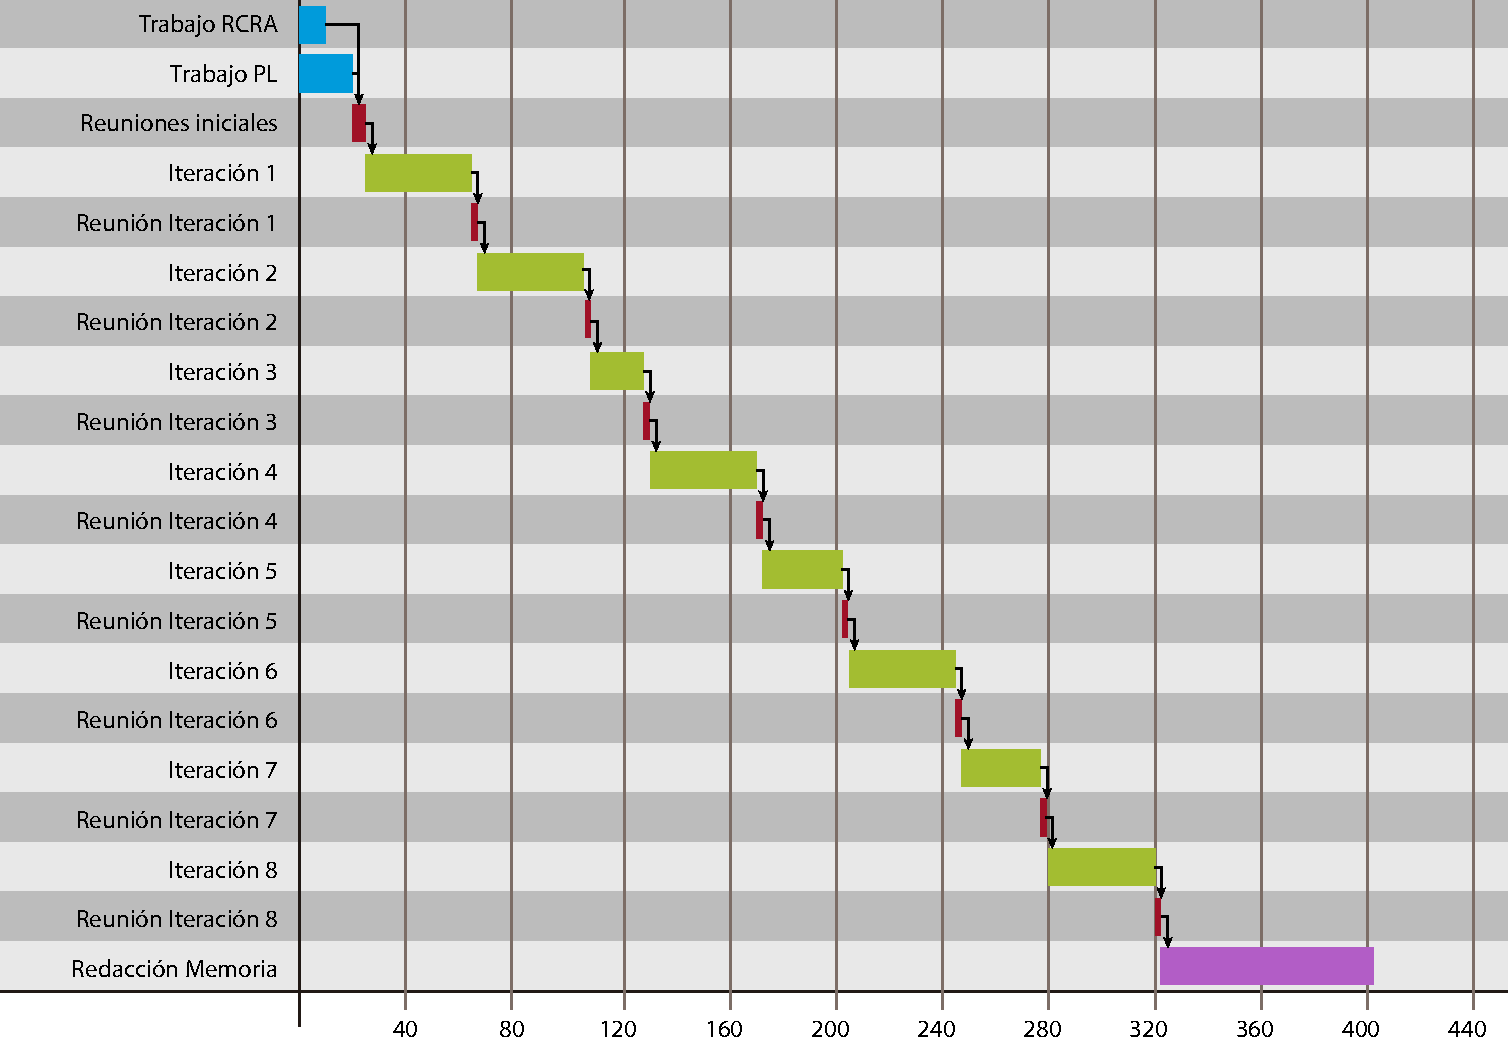
\includegraphics[width=0.7\linewidth]{imagenes/diagrama_tareas.pdf}
		\end{figure}
		
				\begin{table}
				\centering
				\resizebox{0.4\textwidth}{!}{%
					\begin{tabular}{ | l | c | c | c |}
						\hline
						\textbf{Profile} & \textbf{Cost/Hour} & \textbf{Hours} & \textbf{Total} \\ \hline
						Student & 5.5\euro{} & 362 & 1991\euro{} \\ \hline
						Director  & 9\euro{} & 12 & 108\euro{} \\ \hline
						\textbf{Total} & & & 2099\euro{} \\ \hline
					\end{tabular}}
				\end{table}
	\end{frame}

\section{Results}
\begin{frame}
	\frametitle{Overview}
	\tableofcontents[currentsection,subsections,hideothersubsections]
\end{frame}
\subsection{Results Flexibility}
\begin{frame}
	\frametitle{Results Flexibility}
	\begin{center}
		\includegraphics[width=0.8\linewidth]{imagenes/no_cello_plain.png}
		\vfill
		\includegraphics[width=0.4\linewidth]{imagenes/no_grade_one_rule.png}
		\vfill
		\includegraphics[width=0.8\linewidth]{imagenes/no_first_grade.png}
	\end{center}
\end{frame}

\subsection{Conclusions}
		\begin{frame}
			\frametitle{Conclusions}
			\begin{itemize}
				\item<pro@1-> Achieved maximum flexibility
			      \item<pro@1-> Accomplished the main goals of the project and extended some of the functionality
			      \item<pro@1-> The tool produces correct scores in good times
			      \item<con@1-> The interface is pretty poor
			      \item<con@1-> User still needs informatic knowledge to use it
			    \end{itemize}
		\end{frame}

\subsection{Future Work}
	\begin{frame}
		\frametitle{Future Work}
		\begin{itemize}
			\item Improve output and correct tiny representation mistakes
			\item Implement a plugin interface for MuseScore 2 so the tool can be used through the editor itself
			\item Improve detection of weak and strong beats of measure
			\item Detect and use with irregular figures such as duplets or triplets
			\item Research about modulation and implement it in the tool
			\item Improve execution times for the inclusion of new voices
			\item Include rhythmic patterning in the new generated voices
			\item Ask for feedback from professional harmony teachers and polish the tool so it can be used in teaching
		\end{itemize}
	\end{frame}
		
\begin{frame}
\centering
\vfill
\includegraphics[width=0.6\linewidth]{imagenes/anagramaUDC.png}
\vfill
\begin{beamercolorbox}[rounded=true,shadow=true,sep=8pt,center]{title}
\inserttitle \par
\end{beamercolorbox}
\vfill
\begin{beamercolorbox}[leftskip=8cm,center,wd=0.7\textwidth]{author}
\begin{columns}[T]
\begin{column}{.49\textwidth}%
\centering
\insertauthor
\end{column}
\begin{column}{.49\textwidth}%
\centering
\director
\end{column}
\end{columns}
\end{beamercolorbox}
\centering
\vfill
Thank you!
\vfill
\insertdate\par
\vfill
\end{frame}


\end{document} 